%=======================================================================
%
% ------------------------------------------------------------------------
% ------------------------------------------------------------------------
% abnTeX2: Modelo de Trabalho Academico  em conformidade com 
% ABNT NBR 14724:2011: Informacao e documentacao - Trabalhos academicos
% ------------------------------------------------------------------------
%Customização Unoesc
% ------------------------------------------------------------------------
% Autor:  Jonas Alessi(alessi.jonas@gmail.com
% Versão: 10 de Julho 2013.
% Edição: TexStudio
% Codificação: UTF-8
% LaTeX:  abnTeX2
%
%=======================================================================

\documentclass[
	% -- opções da classe memoir --
	12pt,				% tamanho da fonte	
	oneside,          % não imprimir em verso e anverso, oposto do twoside 
	a4paper,			% tamanho do papel. 
	% -- opções da classe abntex2 --
	chapter=TITLE,		% títulos de capítulos convertidos em letras maiúsculas
	section=TITLE,		% títulos de seções convertidos em letras maiúsculas
	subsection=TITLE,	% títulos de subseções convertidos em letras maiúsculas
	%subsubsection=TITLE,% títulos de subsubseções convertidos em letras maiúsculas
	% -- opções do pacote babel --
	english,			% idioma adicional para hifenização
	brazil			% o último idioma é o principal do documento
	,sumario=abnt-6027-2012,
	]{abntex2-unoesc}


% ---
% Pacotes fundamentais 
% ---
\usepackage{cmap}				% Mapear caracteres especiais no PDF
\usepackage{times}			    % Usa a fonte Latin Modern			
\usepackage[T1]{fontenc}		% Selecao de codigos de fonte.
\usepackage[utf8]{inputenc}		% Codificacao do documento (conversão automática dos acentos)
\usepackage{lastpage}			% Usado pela Ficha catalográfica
\usepackage{indentfirst}		% Indenta o primeiro parágrafo de cada seção.
\usepackage{color}				% Controle das cores
\usepackage{graphicx}			% Inclusão de gráficos
\usepackage{amsfonts}			% Símbolos
\usepackage{amsmath}
\usepackage{caption}
\usepackage{enumitem}
\usepackage{pdfpages}
\usepackage{multirow}
\usepackage{multicol}

\setitemize[0]{itemindent=0.4cm,itemsep=0pt}
\setenumerate[0]{itemindent=0.5cm,itemsep=0pt}
%------
% ---
% Pacotes de citações
% ---
\usepackage[brazilian,hyperpageref]{backref}	 					  % Paginas com as citações na bibl

%Referência
\usepackage[alf, 	
			 		abnt-emphasize=bf,
				    abnt-url-package=none,
				    abnt-repeated-title-omit=yes,
				    abnt-full-initials=yes,                                        %yes nome por extenso, no apenas iniciais
					abnt-etal-list=3												%abreviar com mais de 3 autores
]{abntex2/abntex2cite}				 	    									    % Citações padrão ABNT
\usepackage{lipsum}							   								       % para geração de dummy text

%\captionsetup[table]{justification=raggedright}
% Configurações de aparência do PDF final
% alterando o aspecto da cor azul
\definecolor{blue}{RGB}{41,5,195}

% --- 
% Espaçamentos entre linhas e parágrafos 
% --- 
% O tamanho do parágrafo é dado por:
\setlength{\parindent}{1.25cm}
\linespread{1.5}

%Espaçamento depois dos títulos
\setlength{\afterchapskip}{\baselineskip}
% %\setlength{\afterchapskip}{\lineskip}

% Controle do espaçamento entre um parágrafo e outro:
\setlength{\parskip}{0cm}  % tente também \onelineskip

\hangcaption
\captionstyle[\raggedright]{}

%Estava mostrando nas referencias quais paginas estavam sendo referenciadas
\renewcommand{\backref}{}
\renewcommand*{\backrefalt}[4]{}

%Reduzir a fonte do caption
\captionnamefont{\centering\ABNTEXfontereduzida}
\captiontitlefont{\centering\ABNTEXfontereduzida}
%Ajuste nas listas de tabela, ilustrações e quadros
\setlength\cftbeforechapterskip{0pt}
% ---
% compila o indice
% ---
\makeindex
% ---

%----Include da capa é fora do documento 
% ---
% Informações de dados para CAPA e FOLHA DE ROSTO
% ---
\titulo{ESTÁGIO SUPERVISIONADO NA EMPRESA...}
\autor{NOME DO ACADÊMICO}
\local{JOAÇABA}
\data{ANO}
\orientador[ORIENTADOR:]{Nome do Orientador}
%\coorientador{Coorientador 2}
\supervisor[SUPERVISOR:]{Nome do Supervisor de estágio}  % no caso de ser estágio
\instituicao{UNIVERSIDADE DO OESTE DE SANTA CATARINA}
\tipotrabalho{Estágio Supervisionado}
% O preambulo deve conter o tipo do trabalho, o objetivo, 
% o nome da instituição e a área de concentração 
\preambulo{Relatório de estágio supervisionado apresentado ao Curso de Engenharia de Computação, Área de Ciências Exatas e Tecnológicas da Universidade do Oeste de Santa Catarina como requisito parcial à obtenção do grau de bacharel em Engenharia de Computação.}
% ---

%---

\begin{document}
% Retira espaço extra obsoleto entre as frases.
\frenchspacing 

% ----------------------------------------------------------
% ELEMENTOS PRÉ-TEXTUAIS
% ----------------------------------------------------------

%--- CAPA ----
\imprimircapa

% --- FOLHA DE ROSTO
\imprimirfolhaderosto
% \imprimirfolhaderosto* (o * indica que haverá a ficha bibliográfica)






% SUMARIO
\pdfbookmark[0]{\contentsname}{lof}
\tableofcontents*
\cleardoublepage

% ------------------------------------------------------
% ELEMENTOS TEXTUAIS
% ------------------------------------------------------
\textual
% Apresentação
\chapter{APRESENTAÇÃO} %Capítulo sempre em LETRAS MAIÚSCULAS
\label{chap:apresentação}

Apresentar as informações necessárias para o entendimento do local de estágio.

% Atividades Desenvolvidas
\chapter{ATIVIDADES DESENVOLVIDAS} %Capítulo sempre em LETRAS MAIÚSCULAS
\label{chap:atividades}

Mostrar as atividades desenvolvidas no período de estágio. Esta etapa tem que ser coerente ao que foi preenchido no formulário de acompanhamento das atividades desenvolvidas pelo estagiário, o qual deve ser, preferencialmente, preenchido semanalmente.


\section{Exemplo de Seção}
\label{sec:apresentacao}


\begin{equation}
\label{eq:2}
x = \frac{{ - b \pm \sqrt {{b^2} - 4\,ac} }}{{2a}}
\end{equation}

\begin{equation}
\label{eq:1}
\left[ {\begin{array}{*{20}{c}}
	1&0&0\\
	0&1&0\\
	0&0&1
	\end{array}} \right] = I
\end{equation}



A parcela $ \frac{-b}{2a}$ é ...

\subsection{Exemplo subSeção}

\subsubsection{Exemplo subsubsection}

Uma grande dica aqui é a utilização do site \textbf{www.tablesgenerator.com} para geração de tabelas.

\begin{table}[!htpb]
	\centering
	\caption{Título da tabela}
	\label{my-label}
	\begin{tabular}{lcc}
		& \multicolumn{1}{l}{Coluna 2} & \multicolumn{1}{l}{Coluna 2} \\ \hline
		Linha 1 & a                            & b                            \\ \hline
		Linha2  & c                            & d                           
	\end{tabular}
	
	
	\fonte{\citeonline{livro-unoesc}.}
	%  \nota{Exemplo de nota}
	% \nota[Anotações]{Exemplo nota personalizada}
\end{table}

\subsection{Imagens}


\begin{figure}[!htpb]
	\centering
	\caption{Motor de indução trifásico}
	\label{fig:Motores}
	\borda{\includegraphics[scale=0.8]{figuras/motores}}
	\fonte{\cite{NR10}.}
\end{figure}

\section{CITAÇÃO}

Segundo  \citeonline[p. 94]{livro-unoesc},
\begin{citacao}
	``Compreende trecho transcrito que apresenta mais de três linhas; mantém-se o discurso do texto original; destaca-se em blocos, espaço simples,com recuo de 4 cm a partir da margem esquerda, com letra menor que a do texto original;sugere-se usar tamanho 10''.
\end{citacao}

Utilizando outros comando de citação \cite{fitzgerald2014}. Teste de citeonline, segundo \citeonline{LUCKMANN2008}............



%CONCLUSÃO
\chapter{CONCLUSÃO}

\lipsum[1-1]




% ----------------------------------------------------------
% ELEMENTOS PÓS-TEXTUAIS
% ----------------------------------------------------------
\postextual

% ----------------------------------------------------------
% Referências bibliográficas
% ----------------------------------------------------------

\bibliography{referencias}

%Apêndices
%\begin{apendicesenv}

\chapter{TÍTULO DO APÊNDICE A}

Arquivos confeccionados pelo autor do trabalho e que não se encaixam no texto.

 Ex: Deduções matemáticas, dimensionamentos extensos e algoritmos.

\end{apendicesenv}

%Anexos
%\begin{anexosenv}
\chapter{Título do Anexo A}
\label{anexoA}

Arquivos não confeccionados pelo autor do trabalho.
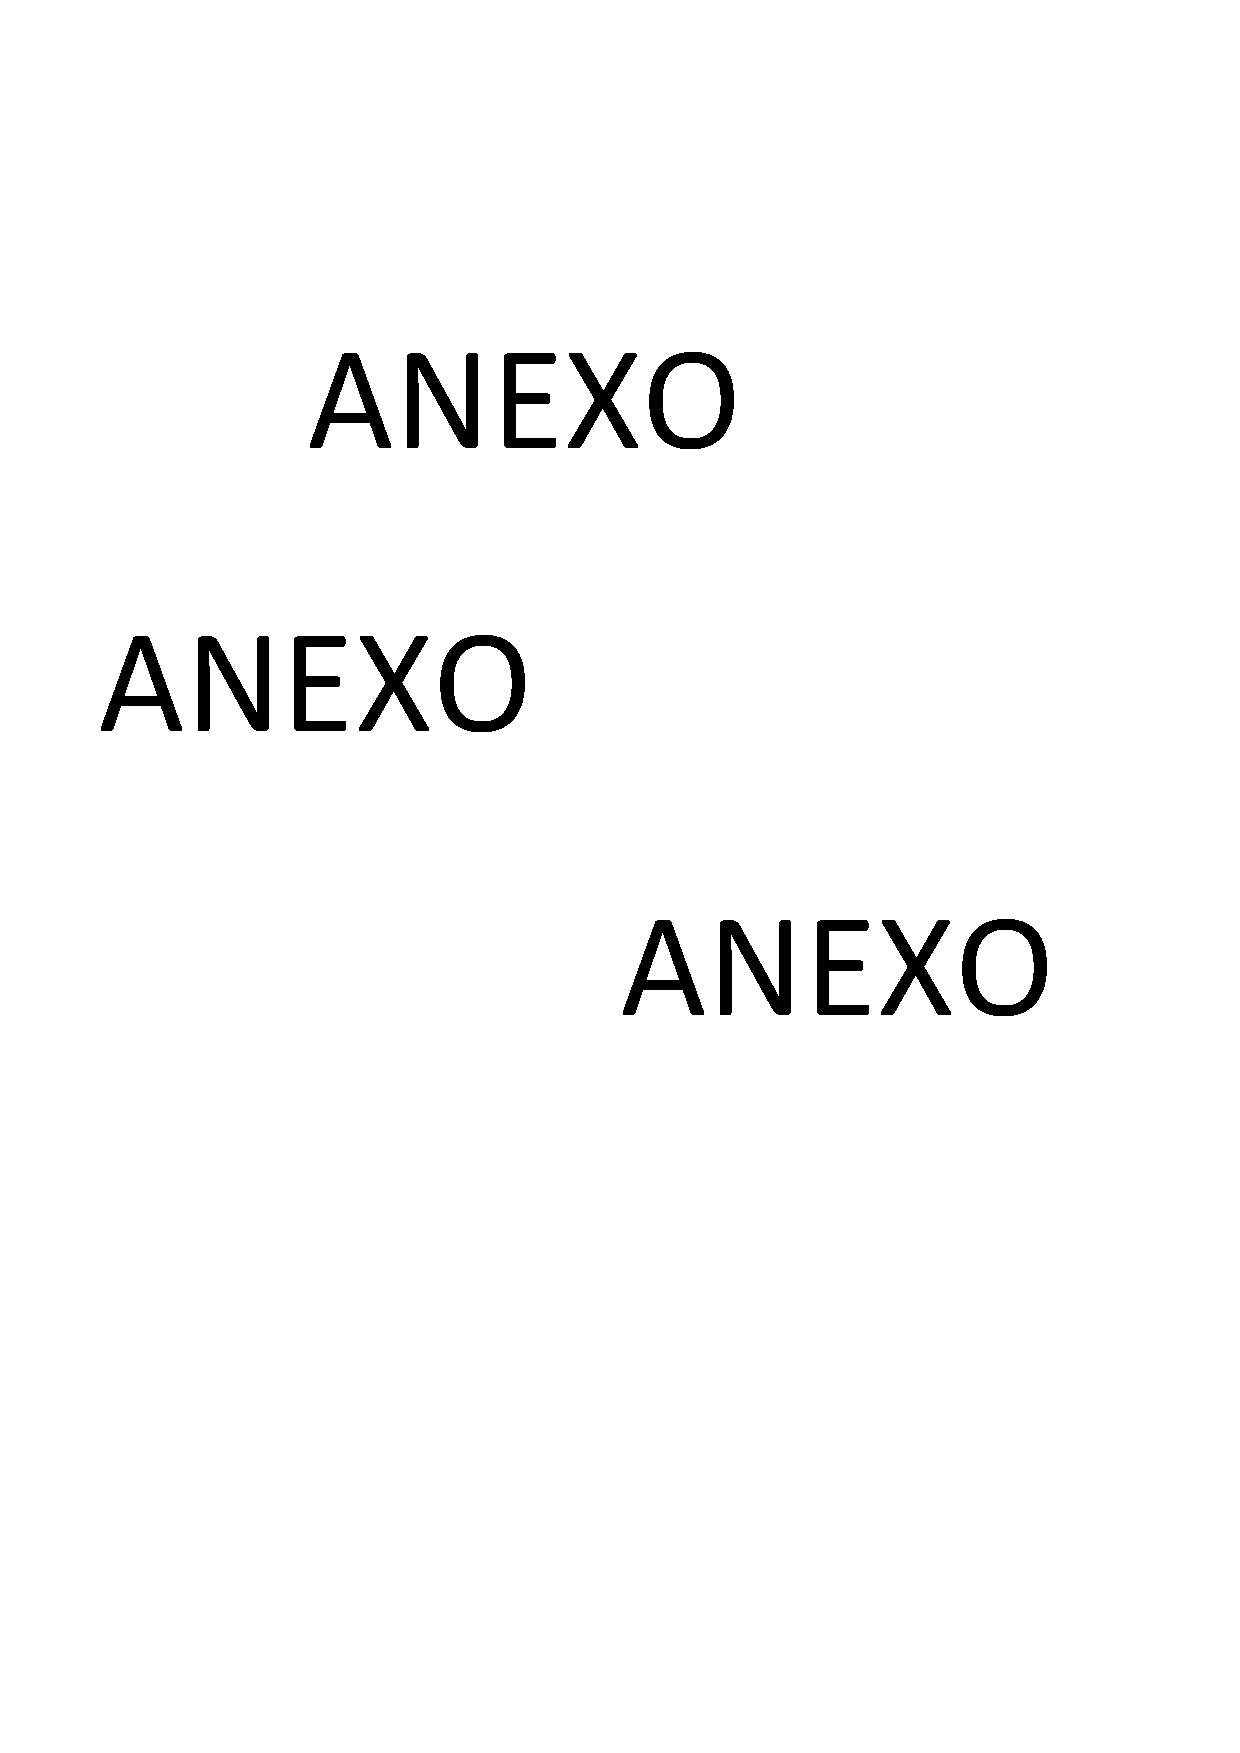
\includepdf{postextuais/anexo1}

\end{anexosenv}

%---------------------------------------------------------------------
% INDICE REMISSIVO
%---------------------------------------------------------------------

%\printindex
\end{document}